\begin{figure}[H]
    \centering
    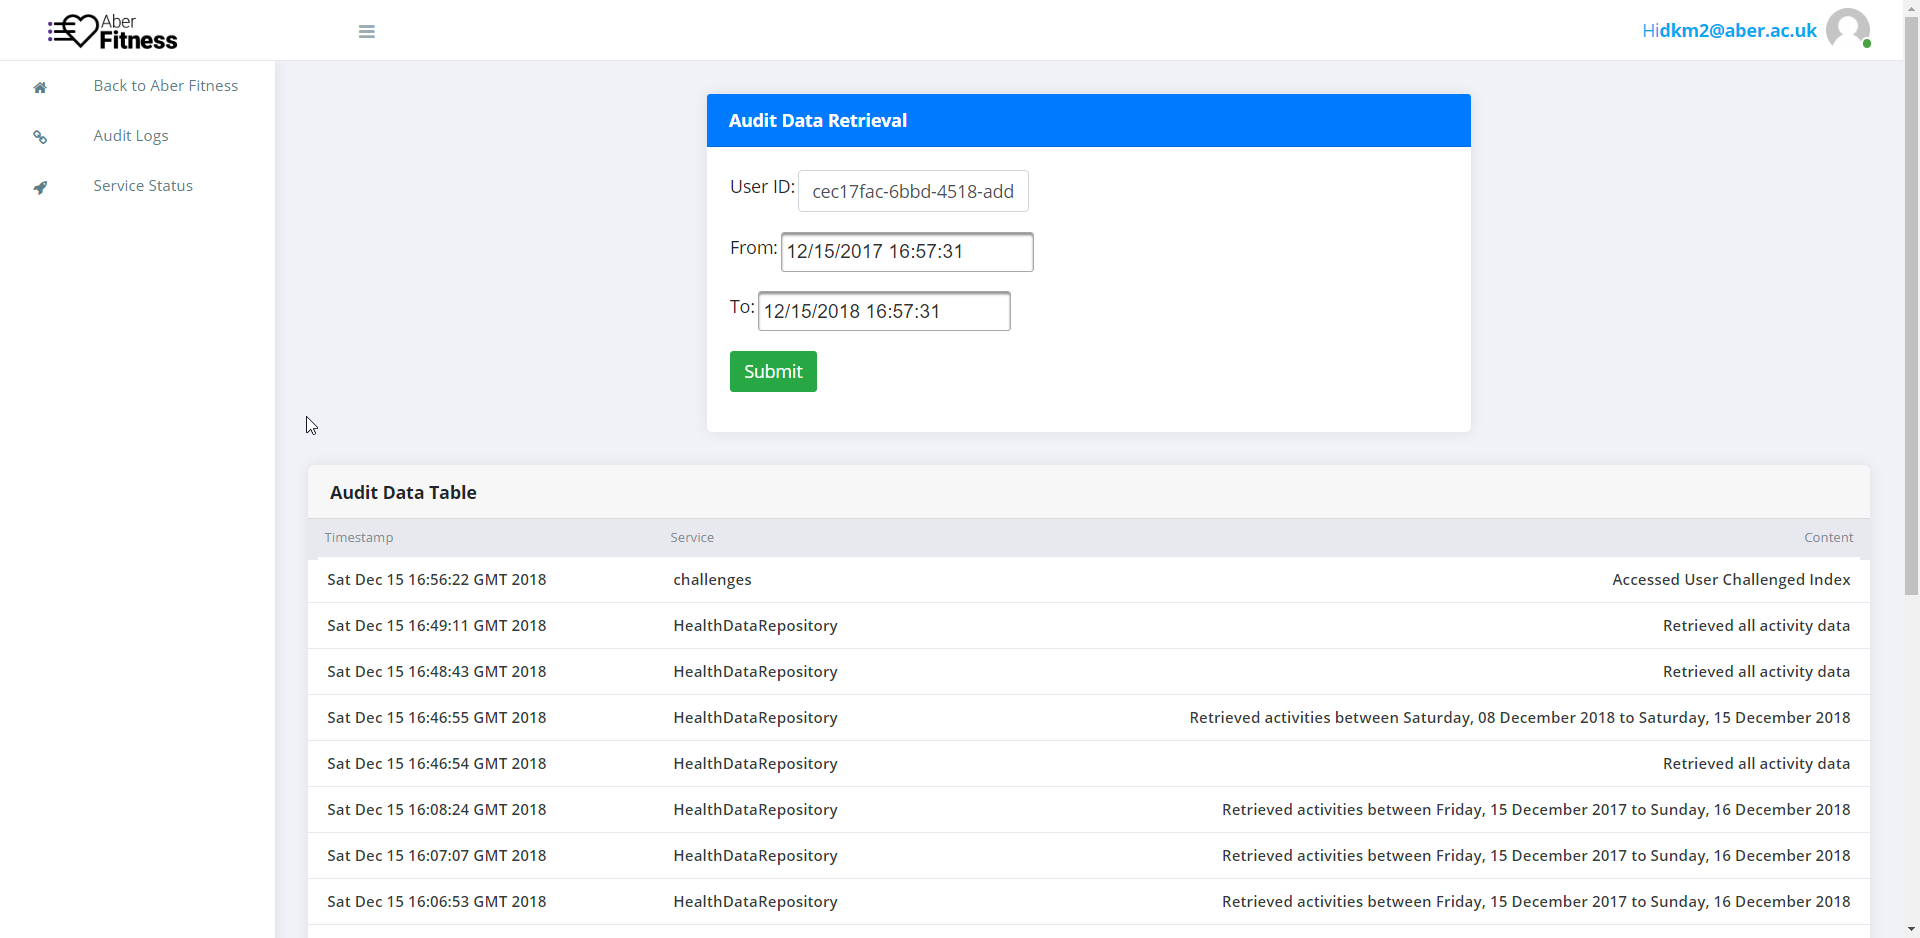
\includegraphics[width=\textwidth]{Images/service_glados.png}
    \caption{A screenshot from GLaDOS displaying a user's audit data, where they can view when and how their data was accessed, modified, or deleted}
\end{figure}

\begin{figure}[H]
    \centering
    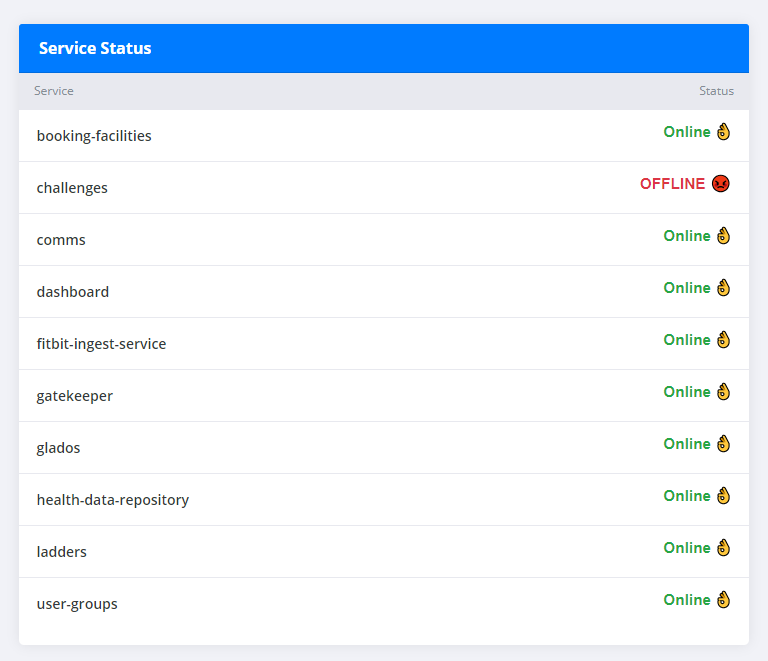
\includegraphics[width=\textwidth]{Images/service_status.png}
    \caption{GLaDOS' service status interface, displaying the status of all the microservices within the system. In this example, the \textit{Challenges} is offline, whereas all other microservices are online}
\end{figure}

\subsubsection{REST API}
\par
The primary role of GLaDOS is to store audit data so that users can view how their data was viewed and modified. Whilst there are native implementations, such as the Java Messaging Service, these require the calls be proxied into a local JVM instance to handle the transport component. We chose to serialise into JSON and use REST as the transport mechanism as all applications had native support for this set up. In addition to this, GLaDOS also offers a page which displays the status of all the microservices within the system.

\par
\textit{JAX-RS} is an API specification for JSON parsing in Java, additionally Payara provides \textit{Jersey} as the implementation of this API at runtime. This avoided us having to package additional dependencies into the web archive. This also allows us to build standard response pages based on the error code internally generated, avoiding having to develop error views.        

\subsubsection{Unit Testing and Mocks}
\par
A new class abstracting the database layer allowed us to avoid writing entity handling at this. We instead focused on writing unit tests which verified the various endpoints correctly serialised or de-serialised data. \textit{Mockito}\cite{Mockito} allows developers to inject mock objects by specifying the class which the test fixture is using.

\par
We could not use dependency injection within the endpoint implementation, as the instantiation point is internal to the framework. This doesn't prevent us from using mocks as Mockito allows a developer to inject them through the reflection methods built into the library. A database call such as `\textit{db.getEntry(id)}' could be tested to see which status codes would be sent and verify the data,if any, was serialised correctly.

\subsubsection{Integration Testing with Arquillian}
\textit{Arquillian}\cite{Arquillian} allows developers to specify the classes to archive and deploy within the text fixture. Payara also provides an embedded Arquillian test container which can be ran at test time to exercise sections of a full system. This would allow us to write integration tests for an end-to-end operations, such as POSTing data to an endpoint and ensuring it is written to the persistence layer.

\par
There was extensive documentation on the methods required to pack an archive, but limited examples on handling Maven dependencies. As the embedded instance provides no runtime methods we were having problems getting the container to correctly run. Developers could specify the full class paths for their dependencies to ensure the were packaged, but this was extremely verbose and fragile.

\par
We looked into using the Maven dependency resolver, which allows developers to get a list of runtime Jars and package them into the archive. However this would led to another set of problems where Maven was trying to export them into a \textit{.zip} format, then throw an exception because this was not supported.

\par
With no easy way to control the format that runtime dependencies were exported in, combined with a lack of documentation pertaining specifically to Maven we agreed to abandon this method of automated testing. This would give us more time for implementing other components within the deadline. We opted to rely on manual integration testing for the duration of the project instead.

\subsubsection{Entity Management}
This service only persists Audit Data, therefore we ultimately need to persist a single entity. Whilst many ORM solutions exists for Java, such as \textit{Hibernate}, we decided against them due to the implementation overhead that was required.

\par
Instead we relied on the persistence layer provided in the EE specification. Using the connection pools which were set up for both Java services (see \ref{JTA_Targets}), we could specify which JTA the injected entity manager should use.

\par
The table schema is managed through annotations on an entity class. This also allows the implementation provided by Payara, \textit{EclipseLink}, to create the tables required at deployment time. As the framework relies on the field types to determine which underlying storage to use there is a hidden pitfall. If the type does not have a native serialisation Java will try to persist this using binary data.

\par
Instants are used to specify timestamps on logs, these are cross compatible as they use \textit{ISO 8601}, a string specifier for absolute time points. This format allows both .NET Core and Java application to send timestamps using the time since POSIX epoch in milliseconds. However as this type was added in JDK 8 there is no native storage conversion built into the entity framework.

\par
Two adaptors were written based on the \textit{AttributeConverter} interface. These provide methods for marshalling and un-marshalling Instants into String objects, which the entity manager can easily store. Annotating the field installed the converting class and correctly updated the schema. This also has the added benefit of making the stored timestamps human readable within the database, which extremely helpful for debugging.

\subsubsection{Developing Facelets}
\par
GLaDOS also provides a page that allows a user to retrieve audit data associated with their account. Administrators can look up any users audit data by user their unique ID too. In addition there is a status page which allows anyone to view the status of all other micro-services without logging in.

\par
The front-end of GLaDOS use facelets to implement the MVC pattern. A backing bean for the user data uses named queries from the persistence layer to retrieve data into a list of entity objects. We switched to using \textit{PrimeFaces}\cite{Primefaces}, which is a fork of the now deprecated \textit{RichFaces}. This allows us to use components such as \textit{DataTables} which dynamically generate tables based on the number of entries returned.

\par
The Fitbit Ingest Service had completed OAuth implementation for connecting to internal and external APIs. This was ported across to GLaDOS and further modified. As the ingest service has no front-end they don't need to persist \textit{JSON Web Tokens (JWTs)}. Additional methods were written specifically for this microservice. These include using the HTTP session handling built into the web framework to persist the token on the server. Another helper class was written which validates the stored JWT as the user navigates through protected pages, or POSTs any requests.

\par
Service statuses were implemented using a singleton Java bean which is instantiated at deployment. Using the scheduling capability provided for EJBs we poll all services every 20 seconds in a seperate thread. All services implement an endpoint at \textit{/api/status} that returns a 200 or 204. This is stored until the page is retrieved where the backing bean, acting as a presenter forward the results on.

\par
As the application stack uses an \textit{nginx} instance to reverse proxy queries the URLs must take this into account when they are generated within the facelet. .NET Core makes this trivial by calling `\textit{App.UsePathBase(URL)}' at start up, however Java applications rely on the context root. This was interfering with the URL rewriting that nginx performs resulting in the service using the 
`\textit{/glados/glados/}' base path.

\par
Initially we used an environment variable to manually generate links between the pages of the service and set the context root to 
`\textit{/}'. However, this quickly proved to be untenable when using forms, as POST requests were being sent to 
`\textit{/destination}' 
rather than 
`\textit{/glados/destination}'. Ultimately to work around this an exception was added to nginx configuration to avoid re-writing any URLs for GLaDOS, and instead rely on the service to correctly address all requests. This allowed us to switch back to generating addresses based on the \textit{outcome} tag and use forms on the service.